% \documentclass{article}
\documentclass[journal,12pt,onecolumn]{IEEEtran}
\usepackage[utf8]{inputenc}
\usepackage{lipsum}
\usepackage{placeins} %(floatbarrier)
\usepackage[colorlinks = true,
            linkcolor = green,
            urlcolor  = blue,
            citecolor = green,
            anchorcolor = green]{hyperref}

\usepackage{graphicx}
\usepackage{caption}
\usepackage{booktabs}
\usepackage{subfig}

\captionsetup{justification=centering}

\usepackage[%
  backend=bibtex      % biber or bibtex
%,style=authoryear    % Alphabeticalsch
 ,style=numeric-comp  % numerical-compressed
 ,sorting=none        % no sorting
 ,sortcites=true      % some other example options ...
 ,block=none
 ,indexing=false
 ,citereset=none
 ,isbn=true
 ,url=true
 ,doi=true            % prints doi
 ,natbib=true         % if you need natbib functions
]{biblatex}
\addbibresource{citations.bib}

\title{Which author do you sound like? \\ Classifying classic authors’ text. }
\author{Tomasz Lewicki (013855803), Kun Su (009437467), Sean Wu (013818714) \\ San Jos{\'e} State Univeristy}


\date{May 2020}

\begin{document}


\maketitle

\begin{abstract}
\noindent In this project we create a dataset of sentences from over 700 books by 20 authors. We obtain the raw texts from Project Gutenberg\cite{gutenberg}, and clean, vectorize and tokenize them in order to obtain dataset. We train and evaluate Neural Network, Naive Bayes and k-NN classifiers, as well as experiment with multiple preprocessing techniques. In this way, we go through the entire standard Data Mining workflow: extract the dataset from a web resource, clean and prepossess the data and finally build several predictive models and evaluate them. Source code is available at \url{https://github.com/tomek-l/cmpe255-data-mining}
\end{abstract}

\section{Introduction}
% Motivation
% Objective
% (Literature/Market review)

Keen readers are often able to identify the author of the text by reading just a short paragraph. Even if they haven't read the exact title, they are able to make a guess inferring from the "style" of writing. But could we train a computer to capture those abstract patterns and perform the same task? Our objective in this project is to classify the author of a book given a short sample of their writing. We were initially inspired by "Spooky Author Identification" challenge\cite{spooky} on kaggle. Unfortunately, the provided sentence dataset contained only 220`000 non-zero values and the objective was to classify texts among 3 authors. Wanting to still pursue this topic, we created a much larger dataset that fulfills the sizing requirement of 50M non-zero values, and allows us to classify texts of 20 authors.

% TODO: Literature review!

\section{Methodology, System Design \& Implementation Details}

% - Algorithm(s) considered/selected (and why)
% - Technologies & Tools used (and why)
% - Architecture-related decisions (if applicable)

\subsection{Approach 1: Naive Bayes Classifier (Kun Su)}
In order to capture each author’s writing style, several methods have been applied to identify the characteristic and unique wording pattern an author might use in his/hers writing. Since an author’s writing habit should be consistent within each sentence, Counter Vectors and TF-IDF are used to detect the frequency or character of the test document while PCA, SVD and select K feature are used to reduce the dimensionality of the feature. Furthermore, Naive Bayes Model uses the term vectors to calculate the probability of one sentence belonging to one each specific author. Lastly, grid search and cross-validation are used to improve and evaluate the model’s performance.

\subsection{Approach 2: Word Embedding Options (Sean Wu)}
General approach to word feature extraction was to vectorize words and transform it into token, however by doing so it discards the meaning between two words let along to paragraphs. By adding an additional layer to the classification model(Doc2Vec), we want to get insight of how two words or two documents relate to each other, and hopefully extract useful information from the corpus and find relevant context to better our classifying models.


\subsection{Approach 3: Convolutional Neural Network (Tomasz Lewicki)}

\subsubsection{Motivation for CNN model}
Convolutional Neural Networks (CNNs) are most commonly known for their application in images, but can be used whenever we aim to capture some spatial pattern in a vector. In theory, CNNs trained on sequences of words may capture the ordering, as well as the relationships between neighboring words in a sample. That characteristic gives a big advantage over other language models that do not preserve ordering (e.g. tf-idf, bag of words), and therefore makes CNNs a compelling candidate for this application.




\subsubsection{Implementation specifics}

I use keras with tensorflow backend for the Neural Network implementation. I train my network an using nvidia GTX1060 GPU. The entire codebase has been also tested on a CPU, but the training will be approximately 7 times slower. For cleaning, data processing and evaluation purposes I use sklearn, pandas and numpy.


% While it's possible to clean most of these in an automated way, book-specific markup is too diverse and inconsistent to reliably deal with. An example of such text is provided in Figure %TODO.
% We therefore black-list some of the particularly difficult texts.


% \begin{figure}
%     \centering
%     \includegraphics{}
%     \caption{Caption}
%     \label{fig:my_label}
% \end{figure}


\

% System (and subsystems if needed) design/architecture/data flow (you may use diagrams with some supportive text)
% Use cases / GUI / screenshots (as applicable)
\section{Data Acquisition \textit{(Tomasz)}}\label{sec:Dataset}

\begin{figure}[t]
    \centering
    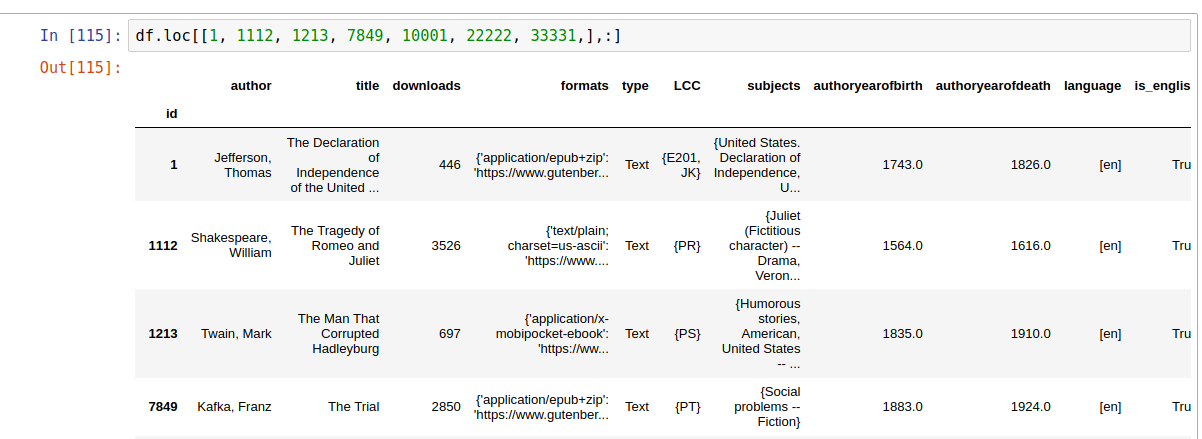
\includegraphics[width=\textwidth]{meta_view.png}
    \caption{View of the meta-index}
    \label{fig:meta_view}
\end{figure}

\begin{figure}[b]
    \centering
    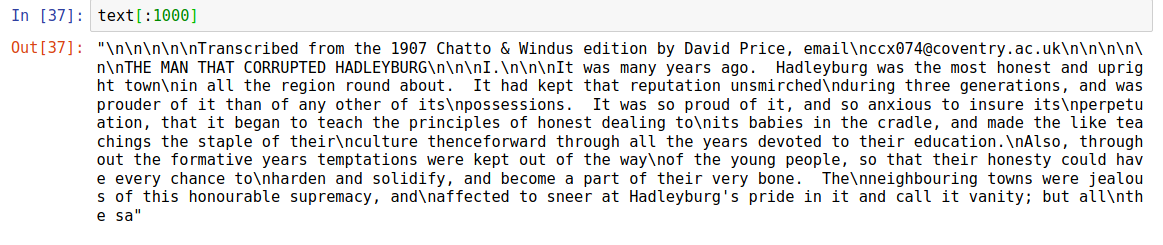
\includegraphics[width=\linewidth]{raw_text.png}
    \caption{Example of raw text (gid = 1213)}
    \label{fig:raw_text}
\end{figure}

\subsection{Dataset Source}

Project Gutenberg is an online library offering over 60'000 ebooks free of charge. It is mainly intended for human users, but also exposes an API for web spiders via \url{http://www.gutenberg.org/robot/}. The texts are not "clean", meaning that they contain additional meta-text, not written by the author of the book. For practical reasons, I do not download all the texts in the Gutenberg Index, but obtain data in a two-step process. First, I download the meta-index (roughly 60 000 titles). Then, I prune the meta-index itself in a manner described in Section \ref{sec:meta}. Lastly, I obtain the unique Gutenberg indices for our authors of interest, and download their books (over 700 titles). 


\subsection{Meta-index cleaning} \label{sec:meta}

Gutenberg meta-index contains information about the texts in the Gutenberg Index. It makes the main index easier to work with, and eliminates the need to download the entire dataset of over 60`000 texts. The meta-index contains some entries that are undesirable from the standpoint of our application, such as:

\begin{itemize}
\item \textbf{Non-textual files}: Most, but not all of the works, are available in UTF-8 text files. However, there are some works that are only available as audiobooks, images, pdfs, etc. I drop these from the meta-index.

\item \textbf{Non-English texts}: While it would be technically possible to include them, I limit the scope of the dataset for practicality. Adding just one new language would roughly double the size of the dictionary. We would then need then need to deal with an increasingly larger vectors for each language we accept. For these reason I only sample books in English.

\item \textbf{Null values}: Some books (around 2400) have a null value in the author. Sometimes it is a data entry error, and sometimes the authors are impossible to establish (e.g. Lascaux Paintings, or old European folk stories). I drop null values.

\item Texts with \textbf{multiple authors}: Some texts have multiple authors (e.g. the Bible). I drop these values. 

\item \textbf{Incorrect indices}: Indices that point to invalid data --- likely introduced to Gutenberg Project by accident.
\end{itemize}

\subsection{Initial Text Cleaning}

\noindent While we preprocess the dataset for the needs of specific models individually, there are certain aspects of the raw data that are objectively undesirable:

\begin{itemize}
    \item Headers, footers
    \item In-text metadata (language, author, file encoding, etc.)
    \item Terms of use and license form Project Gutenberg
    \item Copyright information, and other annotations from the original (printed) book publisher.
    \item The use of whitespaces for to enforce certain page layout.
\end{itemize}
Figure \ref{fig:raw_text} shows an example text prior to any cleaning or preprocessing. The same text is accessible via \url{http://www.gutenberg.org/files/1213/}


\subsection{Final Dataset}
\begin{figure}[h]
    \centering
    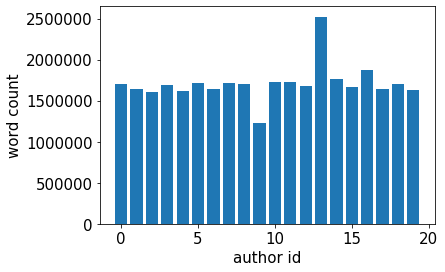
\includegraphics[width=0.5\linewidth]{word_count.png}
    \caption{Dataset classes}
    \label{fig:word_count}
\end{figure}
I sample an equal amount of characters from the corpus by each author. Dealing with characters makes the web scraping part easier, but introduces a slight imbalance in the dataset (authors who use shorter words will have more samples). The word counts per author are depicted in \ref{fig:word_count}. The author who got the fewest samples (id=9) is a British novelist William Wymark Jacobs. The author who has the most samples (id=13) is John Lothrop Motley --- he indeed uses lively language with a lot of verbs, and short words.



% Dataset(s) used (name, source, type of data, size of data, # of instances/statistics, any preprocessing performed etc.)
% Methodology followed (e.g. n-fold-cross validation, number of folds, size of training/test set etc.) (as applicable)
% Graphs showing different parameters/algorithms evaluated in a comparative manner, along with some supportive text. (as applicable)
% Analysis of results
\section{Naive Bayes Classifier - Experiments \textit{(Kun)}}

\subsection{Sentence Preprocessing}
After data cleaning, the text sentence still needs to be preprocessed before the modeling. Since numbers, punctuation, and special symbols in the sentence have no much meaning to represent the "style" of the author, they have been removed by using Regular Expression. In addition, a short phrase such as ”THE END” can come from all possible authors and it is impossible to predict where it comes from. Therefore, we remove common sentences and short phrases where the count of the character is less than the threshold for instance 100 characters. The threshold might vary for different models. Figure-4 showing the distribution where the x-axis is the count of the characters from 0 to 150, and the y-axis is the frequency of the count from 0 to 16000.

\begin{figure}[h]
    \centering
    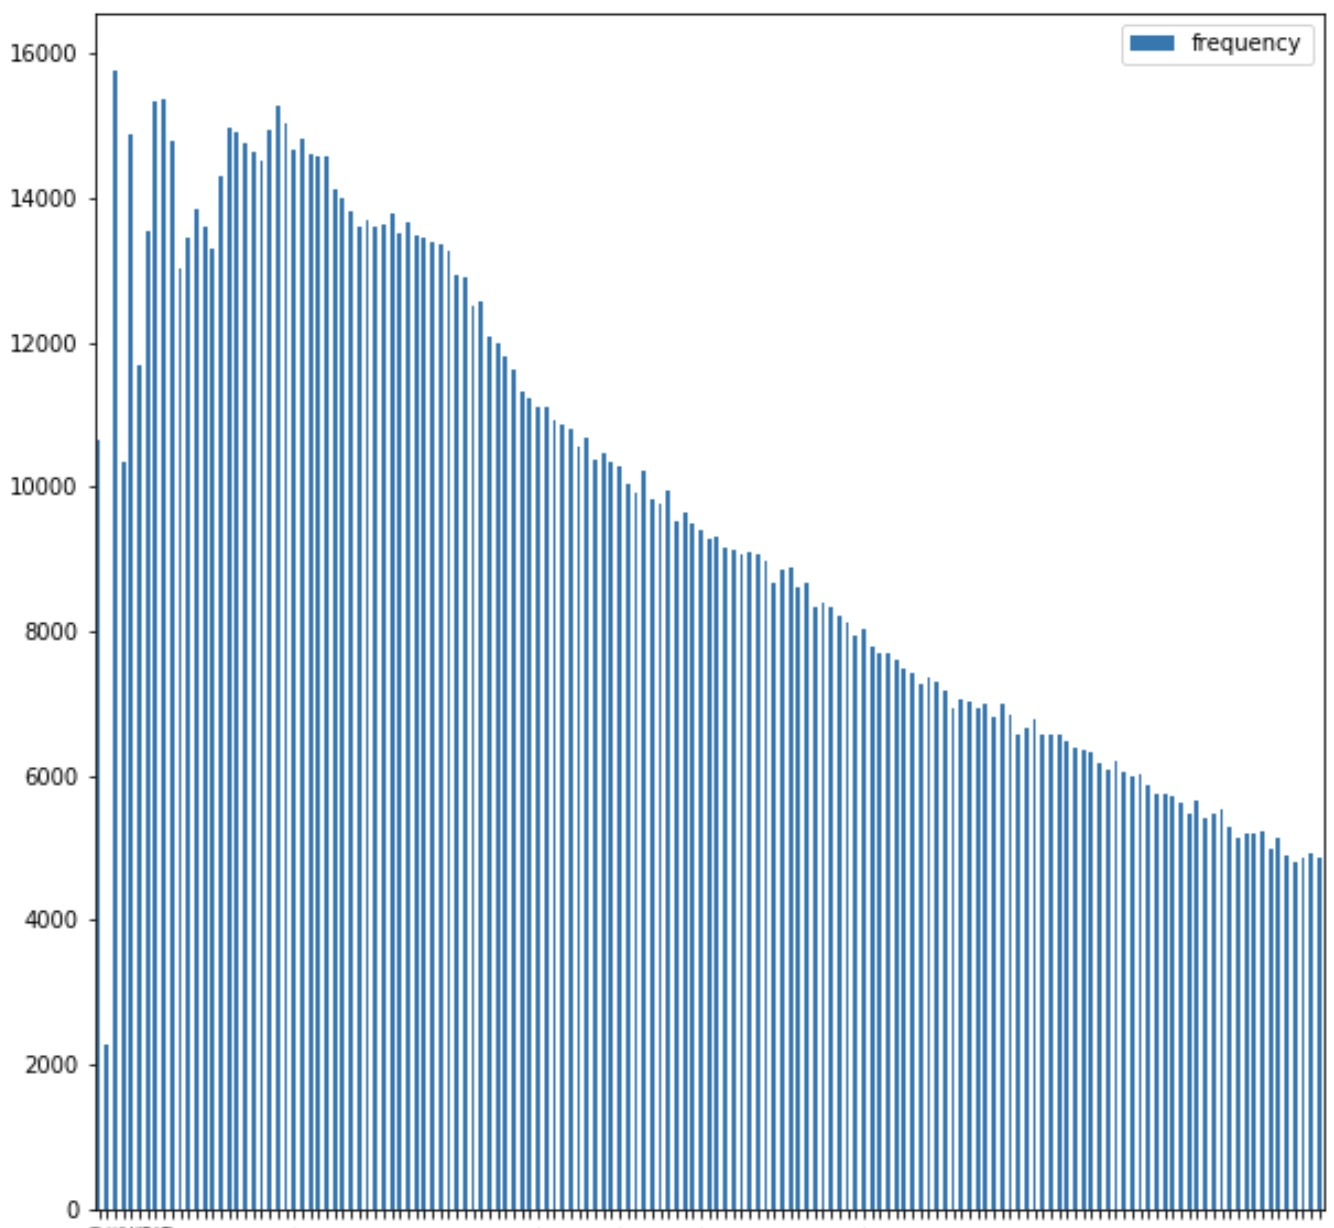
\includegraphics[width=0.5\linewidth]{sentence_distribution.jpg}
    \caption{sentence distribution}
    \label{fig:distribution}
\end{figure}

\subsection{Best sentence length}
By looking at the distribution, we can observe that there are a huge number of short sentences in the dataset. It means we need to lower the threshold as a cutoff to avoid a huge number of data loss. Hence, I did small experiments on picking the best cut off point k as the number of the character counts from the sentence against the accuracy from running a basic Naive Bayes model. With the experiment, the optimized threshold is picked near the pike to maximize the use of the data. 

\begin{figure}[h]
    \centering
    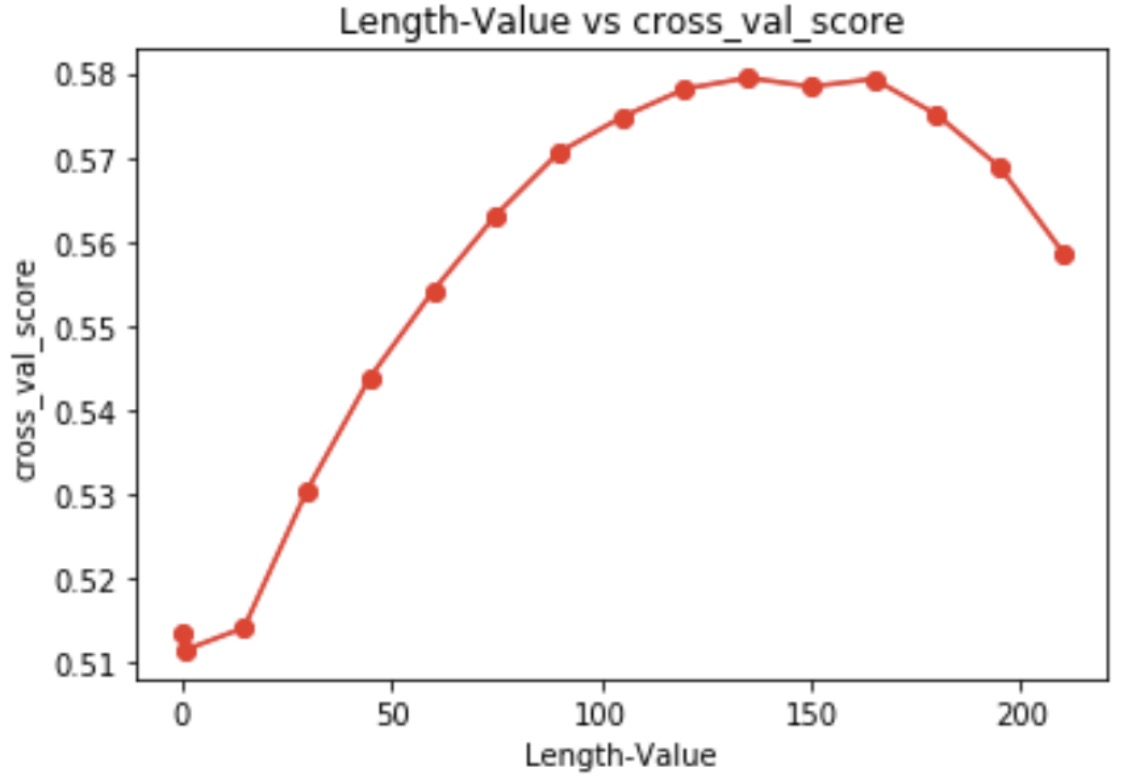
\includegraphics[width=0.5\linewidth]{sentence_length.jpg}
    \caption{sentence length vs accuracy}
    \label{fig:k_length}
\end{figure}

\subsection{Count Vector}
After having the ideal text size, the next step is to convert the text document into count vector. The idea is simply counting each term with its frequency and transforming each document into one set of term frequency vectors. The similarity between two different documents can be calculated based on the cosine similarity of the two documents. However, the top frequent terms are not always a great representation of the author’s writing. multiple authors might have the same high-frequent terms commonly. Therefore, TF-IDF will be the solution to this problem.

\subsection{TF-IDF}
Converting documents into TF-IDF can lower the score of commonly used frequent terms such as stopwords and trending words. However, stopwords are not part of the target representation. A good representation is a set of unique words with a predictable pattern that an individual author always used. Therefore, removing stopwords from the text set will be a good idea. In practice, an interesting finding is that the stopwords from SKLearn \cite{sklearn_tfidf} are different from the stopwords from NLTK \cite{nltk_tfidf}. For instance, the word ”Did” did not filter out by using the stopwords from sklearn. Figure-6 showing the different results by applying different stopwords library.

\begin{figure}[h]
    \centering
    \subfloat[sklearn]{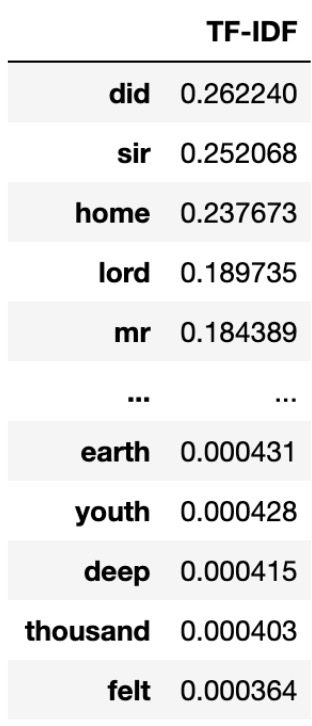
\includegraphics[width=2cm]{stopwords_from_sklearn.jpg} }
    \qquad
    \subfloat[NLTK]{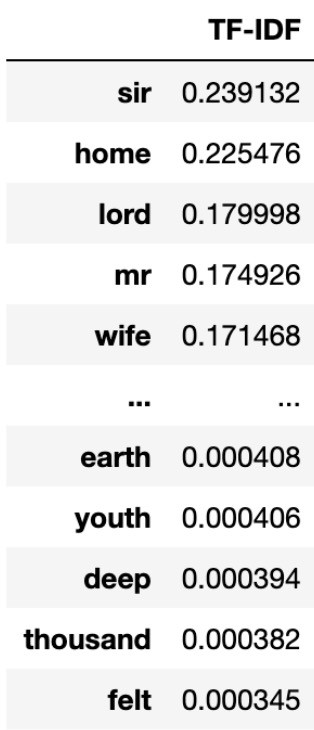
\includegraphics[width=2cm]{stopwords_from_NLTK.jpg} }
    \caption{TF-IDF with different stopwrods}
    \label{fig:example}
\end{figure}

\subsection{Dimensionality Reduction}
After moving stopwords away from the text, there are a total of 2 Million TF-IDF as the features before the modeling. Most of the features have very low variance and lots of them are even close to zero. A feature that is approximately zero will not improve the performance of the model. In this case, those features should be removed. In short, the reason why we are using selectkbest over singular value decomposition (SVD) and principal component analysis (PCA), simply because the selectkbest performs better and computes slightly faster than the other two methods. In addition, it is relevantly easy to find the best k value by trying different k values against the basic model and pick the best-performed k value with less value loss possible in Figure-7.

\begin{figure}[h]
    \centering
    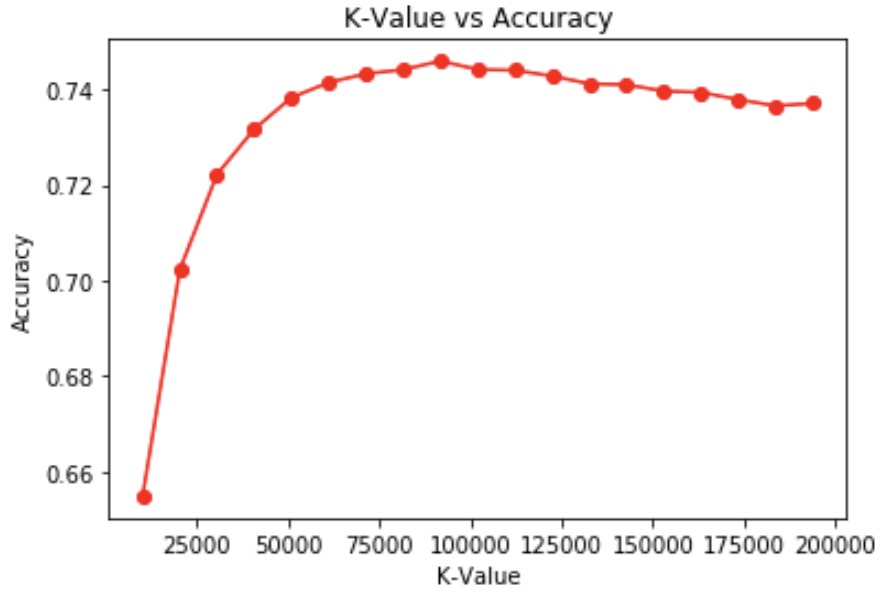
\includegraphics[width=0.50\textwidth]{k_feature.jpg}
    \caption{K-Value vs Accuracy}
    \label{fig:Best K Feature}
\end{figure}

\subsection{Naive Bayes Classifier}
Multinomial Naive Bayes is often used for document classification problems. For example, whether a document belongs to the category of sports, politics, technology, or authors. The features used by the classifier are the frequency of the words present in the document \cite{naive_bayes}. Other models in NaiveBayes Classifier such as Bernoulli Naive Bayes is not suitable for the dataset since it requires boolean variables and same reason with Gaussian Naive Bayes which requires continuous values. Most importantly, the predictors in this dataset are already independent, which fulfills part of the requirement of Naive Bayes modeling. The training and testing data has been split into a 9:1 ratio, where there are 400K training data points with 100K features. After training the base model, we are getting an accuracy of 0.659 with 1.470 in logloss. 

\subsection{Grid Search}
Grid-search is used to find the optimal hyperparameters of a model which results in the most ‘accurate’ predictions \cite{gs}. By applying Grid-search in the Naive Bayes Model, a sample pipeline for text feature extraction and evaluation has been implemented with the inspiration from Olivier's work \cite{grid_search}. A detailed hyperparameters table is shown in Figure-8. After turning from Grid-search, the final model has reached an accuracy of 0.750 with a logloss of 1.056.

\begin{figure}[h]
    \centering
    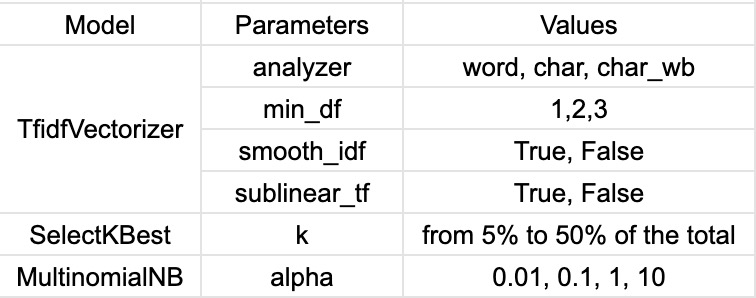
\includegraphics[width=0.5\linewidth]{grid_search.png}
    \caption{Grid Search hyperparameter}
    \label{fig:hyperparameter}
\end{figure}

\subsection{Cross Validation}
Cross-validation is a resampling procedure used to evaluate machine learning models on a limited data sample. The value for k is set to 10,which is found through the earlier experimentation to generally result in a model skill estimate with low bias a modest variance \cite{cv}. The mean score of cross-validation on the final model is similar to the training score, which means the final model is generalized enough to perform without overfitting issue.

%%%%%%%%%%%%%%%%%%%%%%% SEAN %%%%%%%%%%%%%%%%%%%%%%%%%%%%
\section{Doc2Vec - Experiments \textit{(Sean)}}


\subsection{Word2Vec embedding}
Word2Vec is essentially a two layed neural network, it takes large corpus of text and produces a vector space, with each unique word in the corpus being assigned a corresponding vector in the space.
It does so in one of two ways, either using context to predict a target word (a method known as continuous bag of words, or CBOW), or using a word to predict a target context, which is called skip-gram \cite{word2vec}.

\subsection{Doc2Vec embedding}
There are two types of Doc2Vec implementations, thie first one is Distributed Memory Model of Paragraph Vectors (PV-DM) and the second one is Distributed Bag Of Words(DBOW)\cite{doc2vec}.
\subsubsection{PV-DM}
The idea of PV-DM is inspired by word2vec, as every paragraph is mapped into a unique vector and every word is mapped into another unique vector as well, the to vectors are then averaged or concatenated into one. The advantage of the PV-DM method is that this is an unsupervised learning, which means that the vectors that we obtained is through unlabeled dataset. Moreover, the result of this method is is that it captures sematics instead of edit distance of two words, for example, the word "farm" would be more closer to "cow" than "fame".
\subsubsection{DBOW}
Distributed Bag Of Words(DBOW) model is slightly different from the PV-DM model. The main difference is that DBOW transforms paragraphs into vectors without word ordering as it forces the model to predict words sampled randomly from the paragraph.

\subsection{Comparison with tf-idf}
As above mentioned, the Doc2Vec captures the relations between two paragraphs, in contrast tf-idf does not take the meaning of the word into account. By applying Doc2Vec we were able to find interesting relations between two paragraphs
\begin{figure}[h]
    \centering
    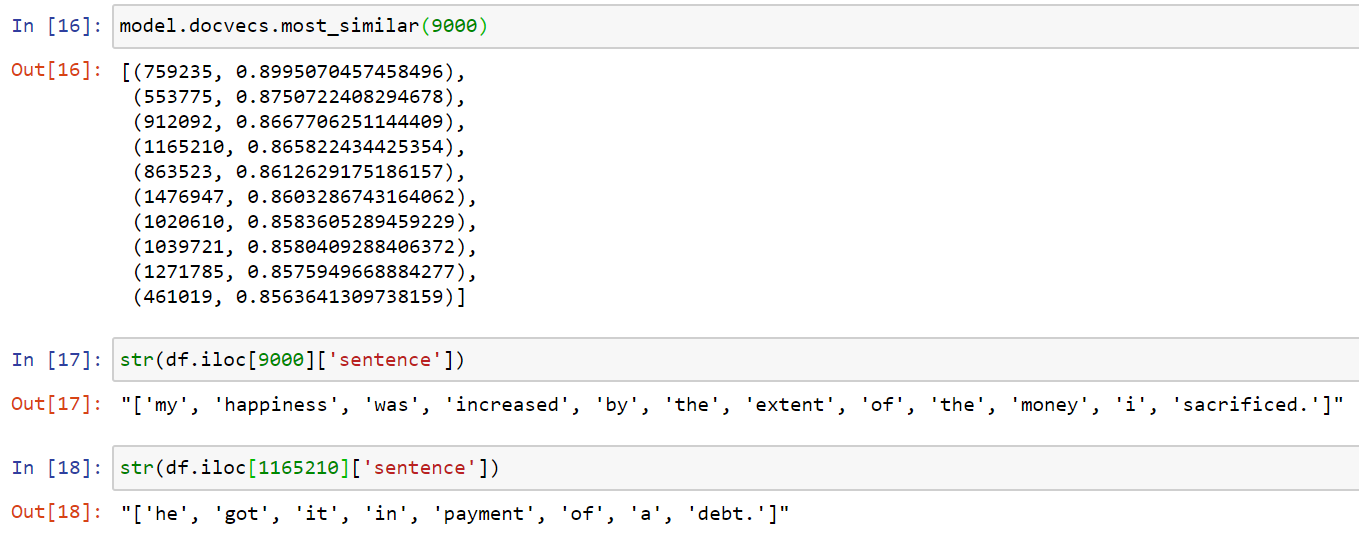
\includegraphics[width=0.6\textwidth]{doc2vec.png}
    \caption{Similar Documents}
    \label{fig:doc2vec}
\end{figure}

%% I(sean) added a new page so that my chart won't get cut into halves

\subsection{Implementation Results}
With this document model we inferred feature vectors from it and plugged it into some classification algorithms using sklearn library.
% Please add the following required packages to your document preamble:
% \usepackage{booktabs}
\begin{table}
\centering
% \Large
\caption{Doc2Vec results}
\label{Doc2Vec results}
\begin{tabular}{@{}cc@{}}
\toprule
Classifier          & Accuracy \\ \midrule
Random Forest       & 0.1286   \\
SVC                 & 0.0895   \\
Logistic Regression & 0.2329   \\
Neural Network      & 0.158    \\ \bottomrule
\end{tabular}
\end{table}
The result of the Doc2Vec was not promising, and by further looking into the data set we concluded with some of the factors that led to this: First is that some of the documents/paragraphs are too short to transform into meaningful feature vectors out of them, which them leads to the second part of the conclusion, the lengths of the corpus is heterogeneous as some of the documents/paragraphs are too long and some of them are too short. By this we could say that the if-idf has the edge over using the Doc2Vec model.


%%%%%%%%%%%%%%%%%%%%%%% SEAN %%%%%%%%%%%%%%%%%%%%%%%%%%%%

\section{Convolutional Neural Net Classifier - Experiments  \textit{(Tomasz)}}

\subsection{Data Preprocessing}

First, I obtain the clean texts as described in Section \ref{sec:Dataset}. Then, I perform the following steps:

\subsubsection{Tokenization} I tokenize the cleaned texts into sparse word vectors. For that purpose, I use the vocabulary of 30`000 words most frequently occurring in the corpus. 

% \subsubsection{Stopwords} I do not remove stopwords. 

\subsubsection{Embedding} I train my own embedding layer, instead of using a pre-trained embedding model. This is a conscious decision. Available pre-trained models such as GloVe or word2vec are usually trained on modern text datasets (e.g. 20 Newsgroup Dataset). A lot of texts in our dataset come from classic authors and use very different vocabulary (e.g. \textit{"If from thy self, to store thou wouldst convert"  --- Shakespeare}). In order to better capture this kind of language, I train my own embedding layer on the obtained dataset.

\subsection{Neural Network Architecture}

I use a Neural Net with architecture reported on the listing below. The key component of this network is a 1D Convolutional layer with kernel size of 3 and 250 filters, acting as a feature extractor. I then use a max pooling layer to reduce dimensionality, and finally use 2 fully connected layers to perfrom the classification. The hidden layers use ReLU activation function, and the output layer uses sigmoid activation.




\begin{figure}[h]
    \centering
    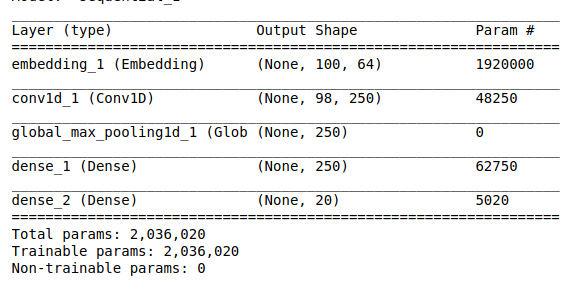
\includegraphics[width=0.5\linewidth]{model.png}
    \caption{Model Architecture}
    \label{fig:model}
\end{figure}


\subsection{Hyperparameter choice}
\subsubsection{Learning rate} I look for the best learning rate for the model. In order to do that, I set up a k-fold cross-validation process, and train the Neural Net for 1 epoch at 20 different learning rates. I choose learning rate with the lowest cross-validation loss after one epoch. The best performing learning rate is ($lr=1.62e-3$). The loss and accuracy curves are illustrated in Figures \ref{fig:acc} and \ref{fig:loss} respectively.

\begin{figure}[!tbp]
  \centering
  \begin{minipage}[b]{0.45\textwidth}
    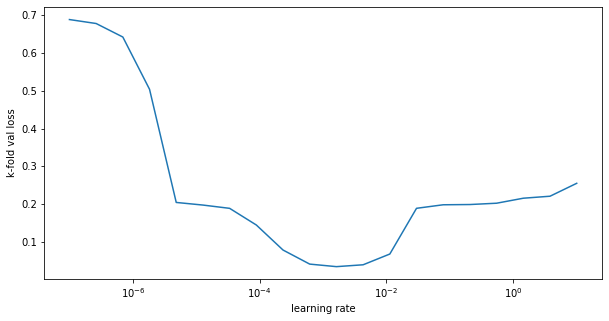
\includegraphics[width=\textwidth]{loss_nn.png}
    \caption{Loss after 1 epoch with varying learning rates}
    \label{fig:loss}
  \end{minipage}
  \hfill
  \begin{minipage}[b]{0.45\textwidth}
    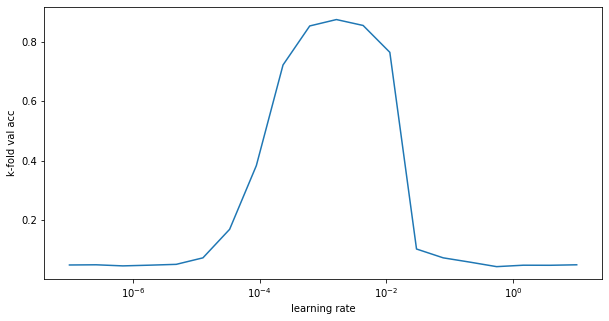
\includegraphics[width=\textwidth]{accuracy_nn.png}
    \caption{Accuracy after 1 epoch with varying learning rates}
    \label{fig:acc}
  \end{minipage}
\end{figure}


\subsubsection{Batch size} I use batch size of 64. This is batch size is optimal in terms of performance on my hardware (nvidia GTX1060 GPU, 1280 CUDA cores). Larger batch size of 128 led to slower model convergence, while providing diminishing speed returns. More performant hardware might be able to benefit from a bigger batch size. The timing results are presented in Table \ref{table:batch}.
 

\begin{table}[h]
\centering
\begin{tabular}{|l|l|}
\hline
batch size & time per epoch \\ \hline
8 & 315s \\ \hline
16 & 139s \\ \hline
32 & 79s \\ \hline
\textbf{64} & \textbf{46 s} \\ \hline
128 & 34 s \\ \hline
\end{tabular}
\caption{Time per training epoch vs batch size}
\label{table:batch}
\end{table}

\subsubsection{Training length}\label{sec:scheduling}
Number of epochs has been tuned by hand by observing the k-fold cross validation accuracy. After 3 epochs, the validation accuracy plateaus, as shown in Figure \ref{fig:plateau}. Further training with the same learning rate will result in \textbf{overfitting} on the train set. Therefore, I reduce the learning rate by a factor of 10, and train for 17 more epochs. The benefit of that approach is presented in Figure \ref{fig:plateau}. 
 

\begin{figure}[h]
    \centering
    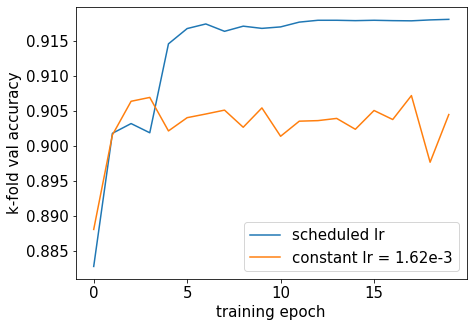
\includegraphics[width=0.5\linewidth]{lr_schedule.png}
    \caption{Positive impact of adjusting lr mid-training}
    \label{fig:plateau}
\end{figure}

\subsection{Metrics}
I use cross-entropy loss function and accuracy to asses the performance of the model. Due to the dimensions of the last layer of the model (20 categorical outputs, one for each class), I use categorical accuracy. Regular (element-wise) accuracy is unfit for tracking the performance --- a classifier predicting all outputs to be 0, would  obtain roughly $1-\frac{1}{n\_classes} = 95\% $ score. For simplicity, I refer to categorical accuracy, as simply "accuracy". I measure all metrics across train, validation and test sets. 


\subsection{Training}
I train the final model for 20 epochs with adam optimizer. For the first 3 epochs, I use $lr = 1.62 \times 10^{-3}$. (as chosen during cross-validation). For the remaining 17 epochs I use $lr=1.62e-4$ for fine-tuning, as described in Section \ref{sec:scheduling}.

\subsection{Performance evaluation}
The best performing model yields accuracy of 92 \% on the test set, with final cross-entropy loss of $7.4 \times 10^{-5}$. The validation metrics track test metrics well. What's very exciting, is that the model seems to generalize well --- in my tests it was able to classify not only the test pieces of the original author, but also texts such as contemporary competition entries mimicking their style.

\FloatBarrier

\section{Discussion \& Conclusions}

Classifying the style in which the text is written is not a trivial task for a computer. Some approaches work better than others. For example, using tf-idf features and a Naive Bayes model did a decent job at predicting the original author (74\% validation accuracy), but it was outperformed by the CNN classifier at 92\% test accuracy. The architecture of the CNN model is still fairly basic, and we believe there's more room for improvement fine-tuning the architecture. Working with any large text dataset, it is especially important to apply techniques that are a good match for the vocabulary we work with. In our example, creating a custom word embedding worked better than using pre-trained embeddings. Finally, it would be an truly interesting experiment to directly compare the performance of our best performing model against an expert human (e.g. a librarian).


% Even though TF-IDF to represent a text document is doing a decent job in predicting the original author, the TF-IDF itself is not able to represent the style of the author. TF-IDF is not able to tell whether the sentiment of a sentence is either positive or negative. An author can use the same word to present different meanings under different scenarios. Therefore, there is a limit to use TF-IDF to predict the author. 

% The dimensionality reduction and grid search work very well on this model. However, the PCA and SVD perform an accuracy loss in the final model, which is  why we use SelectKfeature over those two methods later on. It is difficult to find out the actual meaning of the text and use that information to predict the author. But in fact, that is the future direction of this project by analyzing the tone and sentiment of a sentence and using Deep Learning techniques such as LSTM to predict the author.


% (bullet points as applicable)
% Decisions made
% Difficulties faced
% Things that worked
% Things that didn’t work well
% Conclusion
\section{Project Plan / Task Distribution}

\noindent\textbf{Kun:} Research, selected and confirmed the project topic, and all work related to the Naive Bayes model. \\
\textbf{Sean:} Do2Vec and tf-idf feature comparison, applied to various classification model to examine result. \\
\textbf{Tomasz:} Project choice, dataset acquisition, dataset cleaning, training, hyperparameter tuning, and evaluation of CNN model. \\

% Break into components and clearly explain
% Who was assigned to what task
% Who ended up doing what task (justify as applicable)



\printbibliography

\end{document}
